\documentclass[12pt,a4paper]{article}
\usepackage[utf8]{inputenc}
\usepackage[T1]{fontenc}
\usepackage[spanish]{babel}
\usepackage[top=3cm, bottom=3cm, left=3.5cm, right=3cm]{geometry}
\usepackage{parskip}
\usepackage{titlesec}
\usepackage{enumitem}
\usepackage{booktabs}
\usepackage{array}
\usepackage{longtable}
\usepackage{hyperref}
\usepackage{graphicx}

\titleformat{\section}{\large\bfseries}{}{0em}{}
\titleformat{\subsection}{\normalsize\bfseries}{}{0em}{}

\setlength{\parindent}{0pt}
\setlength{\parskip}{6pt}
%\usepackage[final]{changes}
\usepackage{changes}

%%%%%%%%%%%%%%%%%%%%%%%%%%%%%%%%%%%%%%%%%%%%%
%comando de corrección
\newcommand{\ga}[1]{\textbf{{\color{red}GA: #1}}\\}
%%%%%%%%%%%%%%%%%%%%%%%%%%%%%%%%%%%%%%%%%%%%%

\begin{document}

% ── Portada ────────────────────────────────────────────────────────────────────
\begin{titlepage}
\centering
\vspace*{1cm}

{\Large UNIVERSIDAD NACIONAL DE QUILMES}

\vspace{0.3cm}
{\large Departamento de Ciencia y Tecnología}

\vspace{0.3cm}
{\large Tecnicatura Universitaria en Programación Informática}

\vspace{2.5cm}

{\LARGE \textbf{TURABILITY}}\\[0.5cm]
{\large \textbf{PLATAFORMA INTEGRAL DE TURISMO ACCESIBLE}}\\[0.3cm]
{\large \textbf{E INCLUSIÓN SOCIAL}}

\vspace{2.5cm}

{\large Alumno: Ezequiel Ibarra}

\vspace{0.3cm}
{\large Directora: Dra.\ Gabriela B.\ Arévalo}

\vspace{2cm}

{\large Abril de 2026}

\end{titlepage}

% ── A. Introducción ────────────────────────────────────────────────────────────
\section*{A. Introducción e Importancia del Tema}

El turismo accesible representa una necesidad crítica para la inclusión social de las personas
con discapacidad. En Argentina, según el Instituto Nacional de Estadística y Censos (INDEC),
aproximadamente el 12{,}9\% de la población presenta algún tipo de discapacidad, lo que
equivale a más de 5 millones de personas que enfrentan barreras cotidianas al momento de
planificar un viaje. A nivel global, la Organización Mundial del Turismo (OMT) estima que el
turismo accesible representa un mercado potencial de más de 1.000 millones de personas,
incluyendo adultos mayores y personas con movilidad reducida~[1].

A pesar de su magnitud, la oferta de información turística accesible en línea es fragmentada,
incompleta y en muchos casos inexistente. Los recursos turísticos raramente especifican con
precisión sus condiciones de accesibilidad, y no existen plataformas nacionales que centralicen
esta información de manera estructurada y verificada.

En base a un relevamiento de necesidades del sector turístico accesible realizado por el equipo del proyecto, se desarrolló
\textbf{Turability}: una plataforma digital de turismo accesible con el objetivo
de conectar a turistas con discapacidad con recursos turísticos, profesionales del sector y
paquetes de viaje adaptados a sus necesidades específicas. La plataforma centraliza información
de accesibilidad detallada en cinco dimensiones: motriz, visual, auditiva, cognitiva y dietética,
con más de 200 atributos específicos por recurso.

Entre las experiencias que la plataforma facilita se encuentran: la búsqueda y reserva de alojamientos
con condiciones de accesibilidad verificadas, la contratación de excursiones y actividades culturales
adaptadas, el acceso a gastronomía con opciones dietéticas específicas, la consulta con guías y
profesionales especializados en turismo inclusivo, y la planificación de itinerarios completos
a través de paquetes turísticos diseñados para distintos perfiles de discapacidad. Todo ello
con información estructurada y verificada que permite al viajero tomar decisiones con certeza
y autonomía.

El proyecto obtuvo el primer puesto en el Premio ILAN-AMIA~[2] de Innovación Social, validando su relevancia
en el contexto de la inclusión digital y el turismo accesible a nivel regional. El presente
Trabajo de Inserción Profesional documenta el desarrollo integral de la plataforma y propone
la extensión del sistema mediante dos nuevos módulos: un sistema de suscripciones para
el widget —un componente de software que se incrusta en sitios web de terceros para ampliar
sus funciones— de accesibilidad web Turability Access, y la finalización de la plataforma de
capacitación en línea orientada a prestadores del sector turístico.

% ── B. Estado actual ───────────────────────────────────────────────────────────
\section*{B. Estado Actual del Sistema}

El ecosistema Turability —el conjunto de aplicaciones interconectadas que conforman la
plataforma— está compuesto por los siguientes módulos, desarrollados e implementados
en entorno productivo:
\begin{figure}[h]
  \centering
  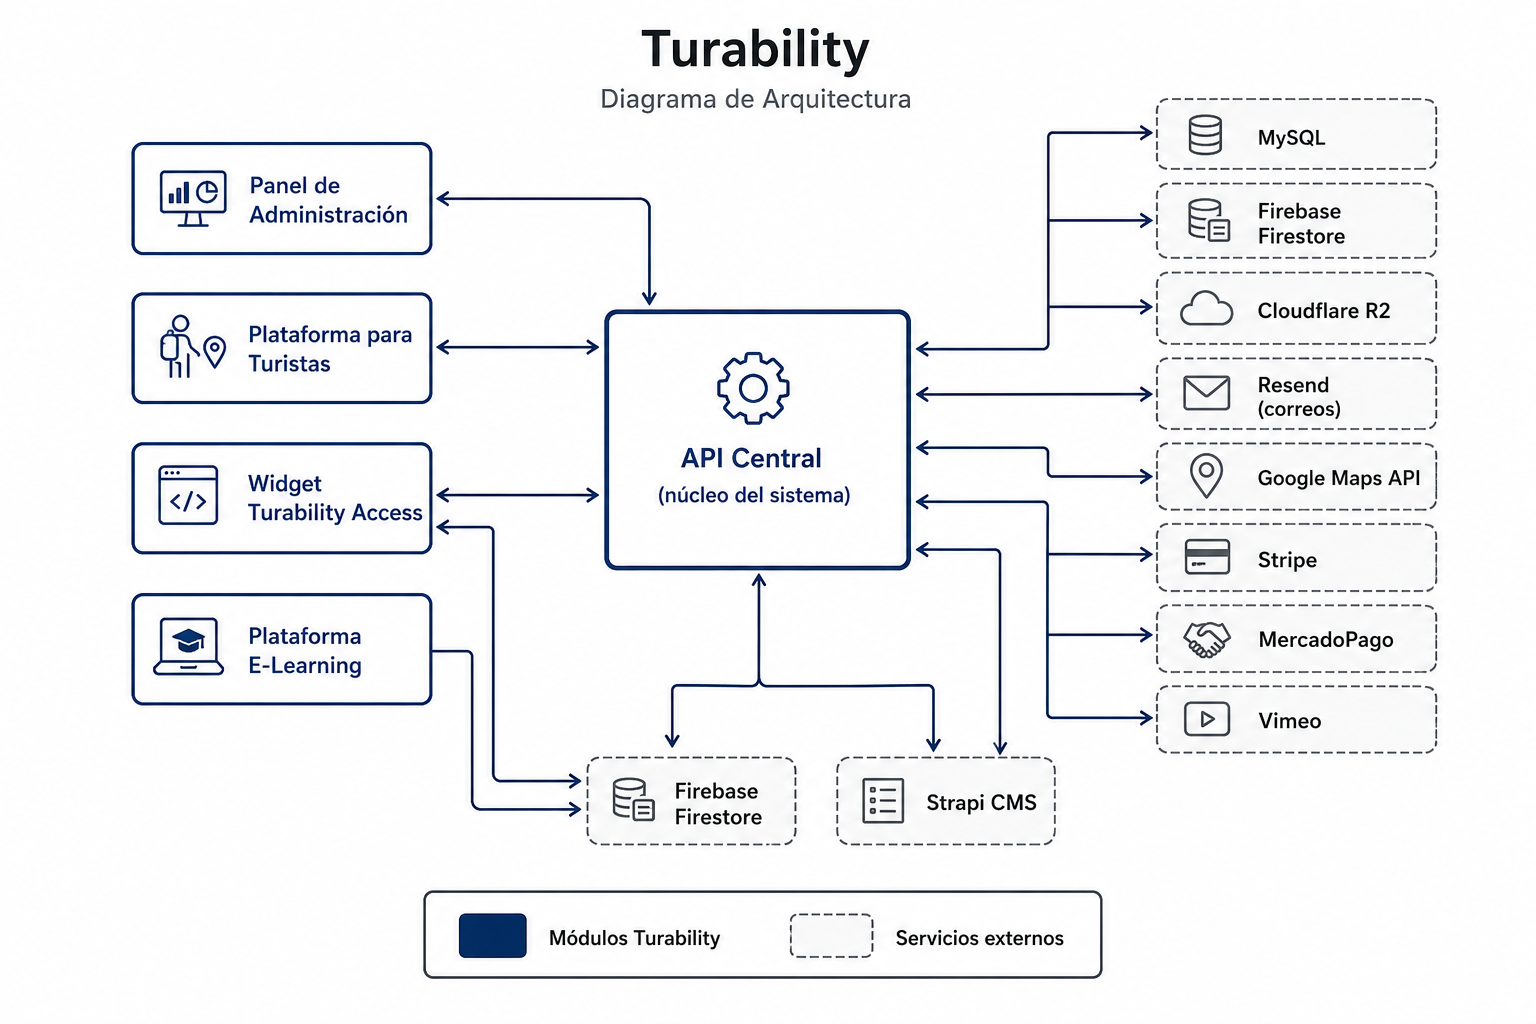
\includegraphics[width=\textwidth]{assets/arquitectura.png}
  \caption{Arquitectura del ecosistema Turability}
  \label{fig:arquitectura}
\end{figure}

\subsection*{B.1 API Central}

La API Central (interfaz de programación de aplicaciones que comunica a los distintos módulos entre sí) es el núcleo del ecosistema Turability: actúa como intermediario entre todos los módulos del sistema, gestionando la lógica de negocio, el acceso a los datos y la comunicación con servicios externos. Es la única fuente de verdad del sistema y el punto a través del cual fluye toda operación, desde el registro de un usuario hasta la validación de una reserva. Técnicamente, es un servidor de aplicación (backend) desarrollado en Laravel~12 con PHP~8.2, que centraliza todos los recursos del
sistema. Incluye autenticación mediante estándares como JWT y Google OAuth, y verificación en dos pasos por código de un solo uso (OTP);
gestión integral —alta, baja, modificación y consulta— de recursos turísticos y profesionales con más de 200 atributos de accesibilidad;
control de acceso basado en roles (RBAC); gestión de reservas, paquetes
turísticos, anunciantes y arquitectura multiinquilino (multi-tenant) que aísla los datos de cada cliente. Se integra con Cloudflare~R2 para almacenamiento
de archivos, Resend para correos transaccionales y la API de Google Maps para geolocalización.
La base de datos principal es MySQL, con Firebase Firestore para módulos específicos como
órdenes, contactos comerciales (leads) y claves de API del widget.

\subsection*{B.2 Panel de Administración}

El Panel de Administración es la herramienta interna con la que el equipo de Turability gestiona el contenido y el funcionamiento de toda la plataforma. Permite administrar recursos turísticos, usuarios, roles, publicidad y reservas desde una interfaz centralizada, con distintos niveles de acceso según el perfil de cada operador. Técnicamente, es una aplicación web desarrollada en Next.js con React, que ofrece una interfaz de gestión diferenciada por rol. Incluye un tablero (dashboard) con estadísticas del sistema; gestión integral de
recursos turísticos, profesionales, usuarios, roles y permisos granulares; administración de anuncios
publicitarios con cuatro ubicaciones publicitarias disponibles; administración de paquetes turísticos y reservas;
sistema de importación masiva de recursos mediante planillas Excel; y gestión de claves de API para el widget
Turability Access. Cuenta con exportación a Excel, diseño adaptable a distintas pantallas, modo oscuro y notificaciones en tiempo
real.

\subsection*{B.3 Plataforma para Turistas}

La Plataforma para Turistas es la cara visible de Turability hacia el público general. Permite a personas con discapacidad buscar y descubrir destinos, alojamientos, actividades y profesionales turísticos con información de accesibilidad detallada y verificada, realizar reservas y planificar sus viajes con la asistencia de una inteligencia artificial. Está diseñada para ser usable por personas con distintos tipos de discapacidad, cumpliendo estándares internacionales de accesibilidad web. Técnicamente, es una aplicación web pública desarrollada en Next.js, orientada al usuario final. Incluye: flujo de
registro e incorporación guiada (onboarding) en cinco pasos con captura del perfil de accesibilidad del viajero;
búsqueda y filtros avanzados de recursos por geografía, categoría y tipo de discapacidad;
detalle de recursos con galería, información de contacto, mapa y sección de accesibilidad;
sistema de reseñas con calificación por dimensión; planificador de viajes mediante una conversación con
la inteligencia artificial ``Abi''; flujo de reservas en varios pasos; favoritos; y perfil de usuario editable. La
plataforma está adaptada para navegación por teclado y lectores de pantalla, cumpliendo
los estándares de accesibilidad ARIA del W3C.

\subsection*{B.4 Widget Turability Access~v1}

Turability Access es una herramienta de accesibilidad web que cualquier sitio puede incorporar para mejorar la experiencia de sus visitantes con discapacidad visual, motriz o cognitiva. Una vez instalado, aparece como un panel flotante que permite al usuario ajustar el comportamiento visual e interactivo del sitio según sus necesidades, sin requerir modificaciones en el sitio huésped. Técnicamente, es un widget embebible en sitios de terceros, desarrollado en JavaScript
puro con Shadow DOM (una técnica que aísla sus estilos para que no interfieran con los del sitio anfitrión). Se integra mediante una única etiqueta de
script —un fragmento de código que el sitio incorpora— autenticada con una clave de API. Implementa doce funcionalidades de accesibilidad
visual e interactiva: ajuste de contraste, saturación, espaciado tipográfico, fuente para
dislexia, cursor ampliado, guía de lectura, máscara de lectura, lectura de texto en voz alta (text-to-speech), pausa de
animaciones, ocultamiento de imágenes, entre otras. Admite cuatro idiomas con detección
automática del navegador y conserva las preferencias del usuario en el almacenamiento local del navegador.
Cuenta con un sistema de validación de claves de API en Firebase Firestore que verifica su actividad,
vigencia y dominios autorizados.

\subsection*{B.5 Plataforma de Capacitación en Línea / E-Learning (versión preliminar)}

La Plataforma de Capacitación en Línea de Turability está orientada a la formación de prestadores y profesionales del turismo accesible. Su propósito es brindar a guías, hoteleros, agencias y otros actores del sector las herramientas conceptuales y prácticas para ofrecer experiencias verdaderamente inclusivas, con certificación digital al finalizar cada programa. Técnicamente, es una plataforma de capacitación en línea (e-learning) desarrollada en Next.js, orientada a prestadores y
profesionales del turismo accesible. Incluye en su versión actual: catálogo de cursos con
precios y filtros; detalle de curso con programa curricular; carrito de compras; proceso de
pago (checkout) por transferencia bancaria; reproductor de video con Vimeo y seguimiento del
progreso; visualizador de documentos (PDF, imagen, Word); cuestionarios (quizzes) con límite de intentos y
devolución inmediata; y el asistente conversacional ``Abi'', integrado tanto en la web como en WhatsApp mediante
Kapso. La plataforma toma su contenido desde Strapi —un gestor de contenidos (CMS)— y registra el progreso del usuario
en Firebase Firestore.

% ── C. Objetivos ───────────────────────────────────────────────────────────────
\section*{C. Objetivos del Trabajo}

\subsection*{Objetivo General}

Consolidar la plataforma Turability como un producto completo, económicamente sostenible y
técnicamente mantenible, incorporando los dos módulos que completan su propuesta de valor: el
sistema de suscripciones del widget de accesibilidad web \textbf{Turability Access} y la finalización
de la \textbf{plataforma de capacitación en línea} orientada a prestadores del sector turístico.

La incorporación de estos módulos es, precisamente, lo que habilita esa sostenibilidad. El
sistema de suscripciones dota al widget de un modelo de negocio que genera ingresos recurrentes
y le permite llegar a sitios de terceros de forma sostenida en el tiempo: en esto consiste la
\textbf{sostenibilidad económica}. A su vez, ambos desarrollos se construyen sobre una arquitectura
documentada y ordenada que asegura su mantenimiento y evolución futura, lo que aporta
\textbf{sostenibilidad técnica}. Por último, la plataforma de capacitación cierra una brecha del propio
producto —la formación de los prestadores del sector—, ya que son ellos quienes, en última
instancia, garantizan que la experiencia accesible que ofrece la plataforma se concrete en la
práctica.

\subsection*{Objetivos Específicos}

\textit{Asociados al sistema de suscripciones de Turability Access:}
\begin{itemize}[leftmargin=1.5cm]
  \item Diseñar e implementar un sistema de planes de suscripción con diferenciación de
        funcionalidades y cuotas de uso.
  \item Integrar una pasarela de pagos que permita la facturación recurrente y automática de
        las suscripciones a nivel global.
  \item Desarrollar un panel de autogestión donde cada cliente administre su suscripción, sus
        dominios autorizados y sus métricas de uso.
  \item Ampliar el conjunto de funcionalidades de accesibilidad del widget y optimizar su
        rendimiento.
\end{itemize}

\textit{Asociados a la plataforma de capacitación en línea:}
\begin{itemize}[leftmargin=1.5cm]
  \item Integrar un medio de pago electrónico que reemplace el flujo manual de transferencia
        bancaria.
  \item Desarrollar un panel de administración propio para la gestión de órdenes, cursos,
        contenidos y usuarios.
  \item Implementar la gestión de personal para empresas, que permita asignar cursos a los
        equipos de trabajo y seguir su progreso.
  \item Completar el sistema de emisión de certificados digitales con validación por código QR.
\end{itemize}

\textit{Objetivos transversales (aplican a todo el trabajo):}
\begin{itemize}[leftmargin=1.5cm]
  \item \textbf{Accesibilidad como requisito de calidad:} garantizar que cada desarrollo cumpla
        los estándares internacionales de accesibilidad web (WCAG~2.1 y ARIA), en coherencia con
        el propósito mismo de la plataforma.
  \item \textbf{Sostenibilidad económica:} dotar a la plataforma de modelos de ingreso —las
        suscripciones del widget y la venta de cursos— que financien su mantenimiento y
        crecimiento.
  \item \textbf{Sostenibilidad técnica:} documentar y sistematizar tanto la arquitectura
        existente como la de los nuevos módulos, para asegurar su mantenibilidad y escalabilidad.
\end{itemize}

\section*{Descripción de Nuevas Funcionalidades}
\subsection*{Sistema de suscripciones y mejoras al widget Turability Access}

El widget Turability Access se encuentra en producción en su primera versión, con validación de
claves de API pero sin diferenciación de planes ni modelo de negocio activo. El objetivo de
este módulo es:

\begin{itemize}[leftmargin=1.5cm]
  \item Implementar un sistema de planes de suscripción (Starter, Pro, Enterprise) con
        diferenciación de funcionalidades y cuotas de uso por plan.
  \item Integrar Stripe como pasarela de pagos recurrentes para la facturación automática
        de suscripciones, permitiendo operaciones a nivel global.
  \item Desarrollar un panel de autogestión para los clientes del widget donde puedan administrar
        su suscripción y sus dominios autorizados, y visualizar sus métricas de uso.
  \item Incorporar analítica de consumo por clave de API: cantidad de veces que se muestra el
        widget, funcionalidades más utilizadas e información de sesión.
  \item Ampliar el conjunto de funcionalidades del widget: perfiles de accesibilidad predefinidos
        (motriz, visual, dislexia, cognitivo), navegación por voz, diccionario en línea y un
        esquema navegable de la estructura de la página (outline).
  \item Optimizar el paquete de código (bundle) que el widget entrega al navegador, reduciendo
        su tamaño para acelerar la carga.
\end{itemize}

\subsection*{Finalización de la plataforma de capacitación en línea}

La plataforma de capacitación se encuentra en una versión preliminar (alpha) con las funcionalidades centrales
implementadas. El objetivo de este módulo es llevar la plataforma a un estado de producción
completo, equivalente a las principales plataformas del mercado:

\begin{itemize}[leftmargin=1.5cm]
  \item Integrar MercadoPago como método de pago principal en el proceso de pago, reemplazando el
        flujo manual de transferencia bancaria.
  \item Implementar el panel de administración de la plataforma con gestión de órdenes, cursos,
        contenidos y usuarios, sin depender de Firebase Console.
  \item Desarrollar un sistema de gestión de personal para empresas, que permita a las organizaciones
        asignar cursos a sus empleados y realizar el seguimiento del progreso grupal.
  \item Implementar cuestionarios de autoevaluación previos al inicio de cada curso para
        personalizar el recorrido de aprendizaje del estudiante.
  \item Completar el sistema de generación y emisión de certificados digitales con validación
        por código QR.
  \item Implementar el flujo de incorporación guiada (onboarding) del usuario dentro de la plataforma.
  \item Mejorar el seguimiento del progreso para incluir los cuestionarios como contenido completable.
\end{itemize}

% ── D. Plan de trabajo ─────────────────────────────────────────────────────────
\section*{D. Plan de Trabajo Propuesto}

\begin{itemize}[leftmargin=0pt, label={}]
  \item \textbf{Mayo 2026 — Junio 2026:} Documentación y sistematización de las funcionalidades
        existentes. Relevamiento técnico y definición de arquitectura para los módulos nuevos.
        Diseño de la base de datos para suscripciones y del flujo de facturación.

  \item \textbf{Junio 2026 — Julio 2026:} Desarrollo del sistema de suscripciones para Turability Access.
        Integración de Stripe para cobros recurrentes a nivel global. Panel de autogestión para clientes
        del widget.

  \item \textbf{Julio 2026 — Agosto 2026:} Mejoras al widget de accesibilidad: nuevos perfiles
        predefinidos, navegación por voz, diccionario y analítica de uso, y optimización del paquete de código.

  \item \textbf{Agosto 2026 — Septiembre 2026:} Finalización de la plataforma de capacitación en línea.
        Integración de MercadoPago en el proceso de pago, panel de administración, sistema de gestión de personal,
        cuestionarios de autoevaluación y certificados digitales.

  \item \textbf{Octubre 2026:} Redacción del informe final. Documentación técnica del sistema.

  \item \textbf{Noviembre 2026:} Presentación y defensa del TIP.
\end{itemize}

% ── E. Decisiones Tecnológicas ────────────────────────────────────────────────
\section*{E. Decisiones Tecnológicas}

La elección del conjunto de tecnologías (stack) responde tanto a criterios técnicos objetivos como a la
experiencia acumulada del autor, priorizando herramientas que permiten avanzar con rapidez
sin resignar robustez ni escalabilidad.

\subsection*{Frontend — Next.js con TypeScript}

El ecosistema de trabajo habitual del autor es JavaScript/TypeScript, lo que hace de
Next.js una elección natural para el frontend (la interfaz y la lógica que se ejecutan del
lado del cliente, en el navegador). Más allá de la familiaridad, Next.js es actualmente el
marco de desarrollo (framework) de referencia para aplicaciones React con renderizado del
lado del servidor (SSR), y ofrece:

\begin{itemize}[leftmargin=1.5cm]
  \item \textbf{Versatilidad de renderizado:} permite combinar SSR, generación de páginas
        estáticas (SSG) y renderizado del lado del cliente según las necesidades de cada ruta,
        algo crítico para una plataforma con contenido público —que debe posicionarse en los
        buscadores (SEO)— y áreas privadas de gestión.
  \item \textbf{TypeScript nativo:} la tipificación estricta con TSX reduce errores en
        tiempo de desarrollo y mejora la mantenibilidad del código a largo plazo.
  \item \textbf{Ecosistema y adopción:} cuenta con amplia documentación, comunidad activa
        y soporte de primera clase por parte de Vercel, lo que garantiza continuidad
        y actualizaciones frecuentes.
\end{itemize}

Alternativas como Nuxt (Vue) o Remix fueron descartadas por tratarse de entornos menos
familiares para el autor y con menor penetración en el mercado al momento del desarrollo.

\subsection*{Backend — Laravel (PHP)}

Para el backend se eligió Laravel, el framework PHP más consolidado del mercado, con más
de una década de desarrollo activo. La decisión se fundamenta en:

\begin{itemize}[leftmargin=1.5cm]
  \item \textbf{Batería de herramientas incluida:} Laravel provee de forma nativa un mapeador
        objeto-relacional (ORM, en este caso Eloquent), sistema de migraciones de base de datos, envío de correos electrónicos,
        colas de trabajo, autenticación y manejo de archivos, entre otros. Esto permite
        avanzar rápidamente sin necesidad de integrar paquetes de terceros para
        funcionalidades comunes.
  \item \textbf{Madurez y estabilidad:} a diferencia de frameworks más nuevos, Laravel
        tiene un historial probado en entornos de producción, con convenciones bien
        establecidas que facilitan el mantenimiento del código.
  \item \textbf{Ecosistema PHP:} el ecosistema PHP cuenta con un enorme conjunto de
        librerías disponibles a través de Composer (su gestor de dependencias) y una amplia base de documentación y recursos
        de la comunidad.
\end{itemize}

Alternativas como Node.js (Express/NestJS) fueron consideradas, pero Laravel ofrece un
nivel de productividad mayor para el tipo de funcionalidades requeridas (facturación,
notificaciones, gestión de usuarios), donde contar con soluciones integradas marca una
diferencia significativa en los tiempos de desarrollo.

% ── F. Lugar ───────────────────────────────────────────────────────────────────
\section*{F. Lugar donde se Realizará el Trabajo}

El trabajo se realizará en la Universidad Nacional de Quilmes, institución en la que el autor cursa
su formación de grado y en cuyo marco académico se desarrolla el presente Trabajo de Inserción
Profesional.

% ── F. Referencias ─────────────────────────────────────────────────────────────
\section*{Referencias Bibliográficas}

\begin{itemize}[leftmargin=0pt, label={}, itemsep=4pt]
  \item {[1]} Organización Mundial del Turismo (OMT). \textbf{Turismo Accesible para Todos}.
        \url{https://www.unwto.org/accessible-tourism}

  \item {[2]} AMIA. \textbf{Premios ILAN-AMIA de Innovación Social}.
        \url{https://amiasocial.amia.org.ar/premios-ilan-amia/}

  \item {[3]} Web Content Accessibility Guidelines (WCAG) 2.1.
        W3C Recommendation, 2018.
        \url{https://www.w3.org/TR/WCAG21/}

  \item {[4]} Faulkner, S. et al. \textbf{HTML: The Living Standard}.
        WHATWG, 2024. \url{https://html.spec.whatwg.org/}

  \item {[5]} Otwell, T. \textbf{Laravel — The PHP Framework for Web Artisans}.
        \url{https://laravel.com/docs/}

  \item {[6]} Vercel Inc. \textbf{Next.js Documentation}.
        \url{https://nextjs.org/docs}

  \item {[7]} INDEC. \textbf{Estudio Nacional sobre el Perfil de las Personas con Discapacidad}.
        Argentina, 2018.
\end{itemize}

\end{document}
